\documentclass{amsbook}

\usepackage[
    a5paper,
    hmargin=28mm,
    vmargin=24mm,
    marginparwidth=18mm,
    marginparsep=3mm
]{geometry}

#PACKAGE_CODE

\title{The First Book. Lucifer in Starlight}

\begin{document}
    \frontmatter
    \renewcommand\thefootnote{{}}
    \maketitle

    \thispagestyle{empty}
    \topskip0pt
    \vspace*{\fill}
    \noindent \textit{The Lord said to Satan, From where have you come? Satan answered the Lord and said, From going to and fro on the earth, and from walking up and down on it...}
    \vspace*{\fill}
    \clearpage

    \tableofcontents

    \thispagestyle{empty}
    \topskip0pt
    \vspace*{\fill}
    {\centering
    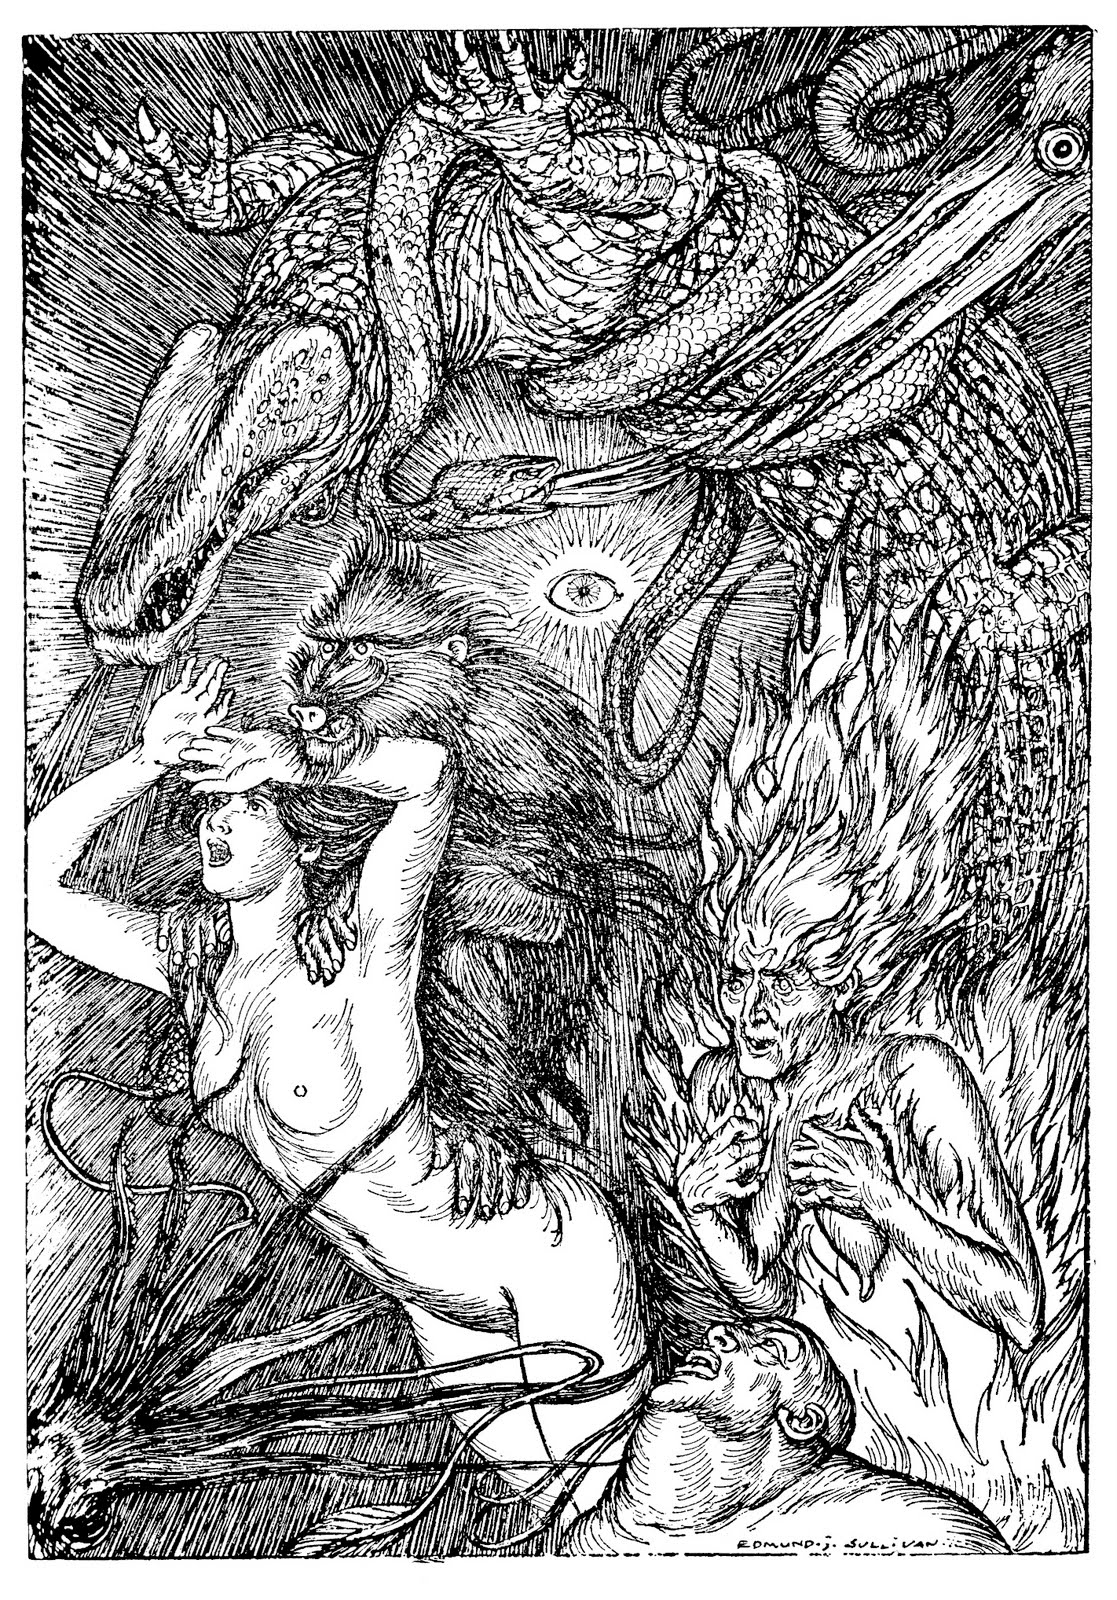
\includegraphics[width=\textwidth]{content/images/rubaiyat.jpg}}
    \vspace*{\fill}
    \clearpage

    \thispagestyle{empty}
    \topskip0pt
    \vspace*{\fill}
    \settowidth{\versewidth}{\vin \vin Around the ancient track marched, rank on rank,}
    \begin{verse}[\versewidth]
        On a starred night Prince \textit{Lucifer} uprose.\\*
        \vin Tired of his dark dominion swung the fiend\\
        \vin Above the rolling ball in cloud part screened,\\
        Where sinners hugged their spectre of repose.\\
        Poor prey to his hot fit of pride were those.\\
        \vin And now upon his western wing he leaned,\\
        \vin Now his huge bulk o'er Afric's sands careened,\\
        Now the black planet shadowed arctic snows.\\
        Soaring through wider zones that pricked his scars\\
        \vin With memory of the old revolt from Awe,\\
        He reached a middle height, and at the stars,\\
        \vin \vin Which are the brain of heaven, he looked, and sank.\nobreak\\
        \vin \vin Around the ancient track marched, rank on rank,\\*
        \vin The army of unalterable law.
    \end{verse}
    \attrib{\textsc{George Meredith} (1828 -- 1909)}
    \vspace*{\fill}
    \clearpage

    \thispagestyle{empty}
    \topskip0pt
    \vspace*{\fill}
    {\centering
    \includegraphics[width=\textwidth]{#AUTUMNAL_IMAGE}}
    \vspace*{\fill}
    \clearpage

    \mainmatter

    \chapter{Autumnal}

    \renewcommand{\poemone}{
        #AUTUMNAL_POEM_1
    }
    \renewcommand{\poemtwo}{
        #AUTUMNAL_POEM_2
    }
    \renewcommand{\poemthree}{
        #AUTUMNAL_PRAYER
    }
    \initprintpoems

    \begin{quote}
        {\footnotesize \textsc{Argument:} How the two lovers from \textit{William's Farewell} -- having suffered an unrecoverable loss -- wandered across England; and the things that happened on their way.}
    \end{quote}
    \bigskip

    #AUTUMNAL_PROSE
    \clearpage

    \thispagestyle{empty}
    \topskip0pt
    \vspace*{\fill}
    {\centering
    \includegraphics[width=\textwidth]{#HIBERNAL_IMAGE}}
    \vspace*{\fill}
    \clearpage

    \chapter{Hibernal}

    \renewcommand{\poemone}{
        #HIBERNAL_POEM_1
    }
    \renewcommand{\poemtwo}{
        #HIBERNAL_POEM_2
    }
    \renewcommand{\poemthree}{
        #HIBERNAL_PRAYER
    }
    \initprintpoems

    #HIBERNAL_PROSE
    \clearpage

    \thispagestyle{empty}
    \topskip0pt
    \vspace*{\fill}
    {\centering
    \includegraphics[width=\textwidth]{#VERNAL_IMAGE}}
    \vspace*{\fill}
    \clearpage

    \chapter{Vernal}

    \renewcommand{\poemone}{
        #VERNAL_POEM_1
    }
    \renewcommand{\poemtwo}{
        #VERNAL_POEM_2
    }
    \renewcommand{\poemthree}{
        #VERNAL_PRAYER
    }
    \initprintpoems

    #VERNAL_PROSE
    \clearpage

    \thispagestyle{empty}
    \topskip0pt
    \vspace*{\fill}
    {\centering
    \includegraphics[width=\textwidth]{#AESTIVAL_IMAGE}}
    \vspace*{\fill}
    \clearpage

    \chapter{Aestival}

    \renewcommand{\poemone}{
        #AESTIVAL_POEM_1
    }
    \renewcommand{\poemtwo}{
        #AESTIVAL_POEM_2
    }
    \renewcommand{\poemthree}{
        #AESTIVAL_POEM_3
    }
    \initprintpoems

    #AESTIVAL_PROSE

    \bigskip
    \bigskip
    \begin{center}
        \textsc{End of the First Book}
    \end{center}

\end{document}
